\documentclass[a4paper,11pt]{article}
\usepackage[utf8]{inputenc}
\usepackage[T1]{fontenc}
\usepackage{graphicx}

\title{Rapport : Implémentation des Entrées/Sorties dans NACHOS}
\author{MAHDI Yanis, LUBET Damien}
\date{\today}

\begin{document}

\maketitle
\tableofcontents


\section{Bilan}
Dans le cadre de ce projet, nous avons implémenté l'ensemble des fonctionnalités demandées pour la gestion des entrées/sorties dans le système d'exploitation Nachos excepté la récupération de la valeur de retour return n. L'objectif principal était de mettre en place des appels systèmes permettant de gérer les entrées/sorties de manière synchrone et asynchrone.
Plusieurs fonctionnalités ont été développées, notamment les appels systèmes pour les fonctions essentielles telles que \texttt{PutChar} et \texttt{GetChar}, permettant respectivement l'écriture et la lecture de caractères via la console. Nous avons également implémenté des mécanismes de gestion des chaînes de caractères avec l'appel \texttt{PutString}.
Tous les appels systèmes requis sont fonctionnels, y compris ceux permettant de gérer les caractères en mode utilisateur, avec une gestion correcte des interruptions. 
Cependant, la dernière partie bonus concernant l'implémentation d'un appel système \texttt{printf} n'a pas été réalisée par manque de temps. 
Mais toutes les autres fonctionnalités essentielles ont été mises en place avec succès et passent les tests conçus pour valider leur bon fonctionnement.



\section{Points délicats}

Parmi les aspects les plus complexes que nous avons rencontrés lors de l'implémentation, l'appel système \texttt{PutString} a été l'un des plus exigeants. 
En effet, la gestion des chaînes de caractères posait un défi lorsqu'elles dépassaient la taille maximale du tampon que nous pouvions lire à chaque itération. 
Pour résoudre ce problème, nous avons dû implémenter une boucle \texttt{while} permettant d'écrire la chaîne morceau par morceau, en continuant jusqu'à ce que nous 
rencontrions le caractère de fin de chaîne (\texttt{\textbackslash0}). Cela garantissait que toutes les chaînes, même les plus longues, étaient correctement écrites, sans provoquer de dépassement de tampon.

Un autre point délicat concernait la gestion de la fonction \texttt{main()} et la manière de prendre en compte la valeur de retour \texttt{return n}. 
Nous avons eu des difficultés à comprendre comment récupérer et traiter cette valeur correctement afin de garantir que le programme utilisateur puisse se terminer sans erreurs. 
On a cependant pas pu trouver la valeur de retour de la fonction \texttt{main} malgré le fait que l'on sache qu'elle se trouve dans le registre \texttt{R2}.

La gestion de l'appel système \texttt{GetString} a également posé problème concernant les débordements notamment coté utilisateur. Nous avons dû faire attention à ne pas consommer plus de caractères que nécessaire, 
tout en garantissant que les caractères restants soient toujours disponibles dans le flux d'entrée pour d'éventuels appels supplémentaire de la fonction. Cela impliquait de ne pas vider le flux immédiatement, 
mais seulement lors de la terminaison du programme, afin d'éviter que des caractères indésirables ne soient renvoyés au shell. 
Pour cela, on a ajouté une variable globale booléenne \texttt{checkflux} qui permet de savoir s'il reste des caractères à lire dans le flux d'entrée ou non. 
Quand c'est le cas, on appelle une fonction \texttt{clearStdin} qui vide le flux d'entrée avant de terminer le programme.
Cela avoir une fonction getString similaire à la fonction fgets dans son comportement.



\section{Limitations}

Un des désavantages de notre implémentation est celle de fonction \texttt{GetString} qui n'est pas adapté pour l'utilisation de threads. 
L'appel de la fonction par plusiers threads en même temps peut conduire à des comportement imprévisibles tels que des lectures incorrectes ou des pertes de données.
Pour remédier à cela, on aurait pu ajouter des mutex pour garantir l'accès exclusif à la fonction \texttt{GetString} à un seul thread à la fois.

\section{Tests}

Nous avons conçu plusieurs tests pour valider le bon fonctionnement de nos appels systèmes.
Le code source des tests contient tous les commentaires nécessaires pour les exécuter avec les bons paramètres et pour connaître la sortie normale attendue à l'écran.


\subsection{Stratégie de test pour PutChar}

Pour valider le bon fonctionnement de l'appel système \texttt{PutChar}, nous avons conçu une série de tests couvrant différents scénarios d'utilisation. L'objectif est de s'assurer que \texttt{PutChar} fonctionne correctement dans des conditions variées.
Voici les tests effectués :

\begin{itemize}
    \item \textbf{Test de l'écriture d'un seul caractère}
    \item \textbf{Test de l'écriture de plusieurs caractères} 
    \item \textbf{Test de l'écriture d'un caractère spécial}
\end{itemize}


\subsection{Stratégie de test pour PutString}

Pour valider le bon fonctionnement de l'appel système \texttt{PutString}, nous avons conçu une série de tests couvrant différents scénarios d'utilisation. L'objectif est de s'assurer que \texttt{PutString} fonctionne correctement dans des conditions variées.
Voici les tests effectués :

\begin{itemize}
    \item \textbf{Test de l'écriture d'une chaîne de caractères courte}
    \item \textbf{Test de l'écriture d'une chaîne de caractères longue dépassant la taille du buffer} 
    \item \textbf{Test de l'écriture d'une chaîne de caractères contenant un caractère de fin de chaîne au milieu}
    \item \textbf{Test de l'écriture d'une chaîne de caractères vide}
\end{itemize}

\subsection{Stratégie de test pour GetChar}

Le test de \texttt{GetChar} est assez simple, il suffit de vérifier que la fonction retourne bien le caractère saisi par l'utilisateur.
Le programme fonctionne de la manière suivante : il demande à l'utilisateur de saisir un caractère, puis affiche le caractère saisi à l'écran tant que le caractère saisi n'est pas q ou CRTL+D (EOF).
Nous avons testé plusieurs cas :

\begin{itemize}
    \item \textbf{Test de la saisie d'un seul caractère}
    \item \textbf{Test de la saisie de plusieurs caractères} 
    \item \textbf{Test de la saisie d'un caractère spécial} 
\end{itemize}


\subsection{Stratégie de test pour GetString}

Le test de \texttt{GetString} est similaire à celui de \texttt{GetChar}, sauf qu'ici on ne fait pas de boucle. 
On teste la saisie d'une seule chaîne de caractères par l'utilisateur.
Le programme fonctionne de la manière suivante : il demande à l'utilisateur de saisir une chaîne de caractères, puis affiche la chaîne saisie à l'écran.
Nous avons testé plusieurs cas :

\begin{itemize}
    \item \textbf{Test de la saisie d'une chaîne de caractères courte} 
    \item \textbf{Test de la saisie d'une chaîne de caractères longue} : On teste la saisie d'une chaîne de caractères plus grande que la taille du buffer pour vérifier que la fonction \texttt{GetString} récupère correctement le bon nombre de caractères demandé par \texttt{getString} sans déborder par la suite dans le shell pour les caractères restants de la chaîne.
    \item \textbf{Test de la saisie d'une chaîne de caractères vide}
\end{itemize}

\subsection{Stratégie de test pour PutInt et GetInt}

La stratégie de test pour \texttt{PutInt} est similaire à celle de \texttt{PutChar} tandis que celle de \texttt{GetInt} est similaire à celle de \texttt{GetString}.




% \begin{figure}[h]
%     \centering
%     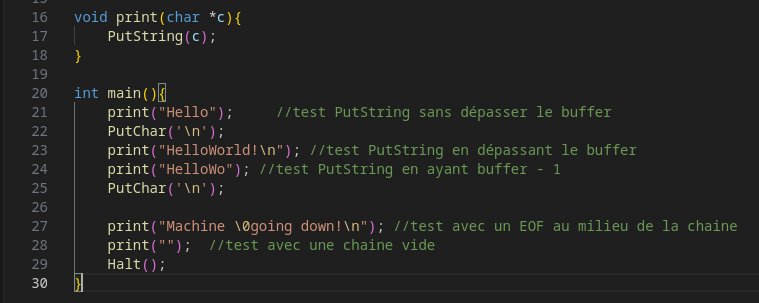
\includegraphics[width=0.9\textwidth]{../images/putstring_marche.png}
%     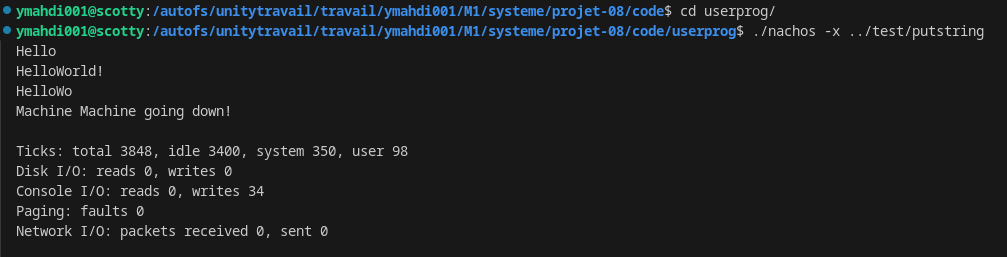
\includegraphics[width=0.9\textwidth]{../images/putstring_marche2.png}
%     \caption{Tests pour vérifier le bon fonctionnement de \texttt{PutString} dans tous les cas.}
% \end{figure}

% \begin{figure}[h]
%     \centering
%     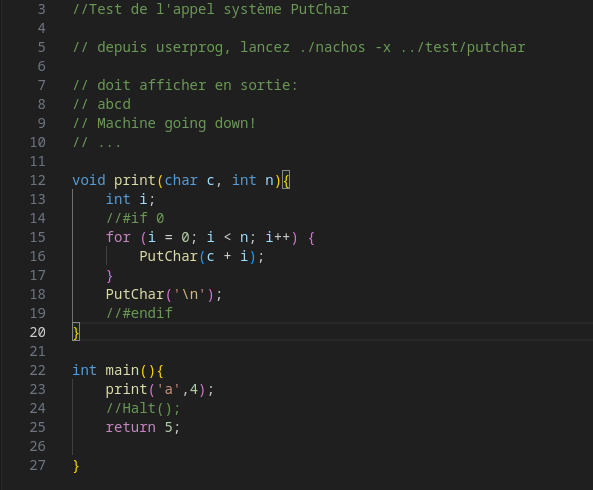
\includegraphics[width=0.9\textwidth]{../images/putchar_test1.png}
%     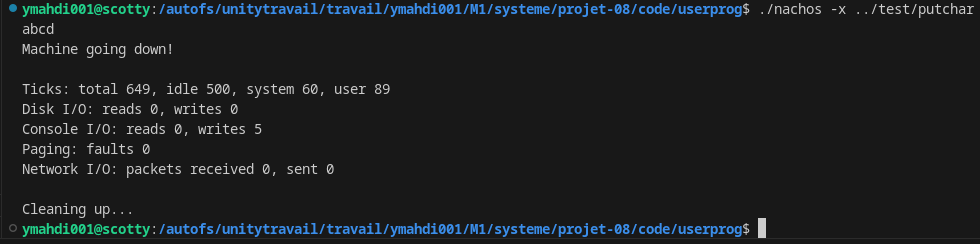
\includegraphics[width=0.9\textwidth]{../images/putchar_test2.png}
%     \caption{Tests pour vérifier le bon fonctionnement de \texttt{PutChar} sans le Halt().}
% \end{figure}

% \begin{figure}[h]
%     \centering
%     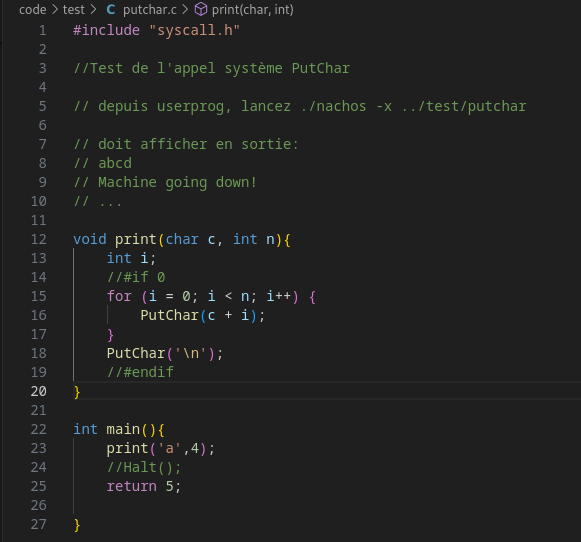
\includegraphics[width=0.9\textwidth]{../images/stop_putchar.png}
%     \caption{Comment s'arrêter sans le Halt().}
%     Pour s'arrêter dans \texttt{putchar.c} sans le Halt(), on a simplement retourner l'entier 5 (ou n'importe quel entier d'ailleurs), tout en implémentant l'exception Exit dans \texttt{exception.cc}.  

% \end{figure}





\end{document}
